\documentclass{exam}
\usepackage[utf8]{inputenc}
\usepackage{lmodern}
\usepackage{microtype}

% \usepackage[parfill]{parskip}
\usepackage[dvipsnames]{xcolor}
\usepackage{amsmath}
\usepackage{amsfonts}
\usepackage{amsthm}
\usepackage{siunitx}
\DeclareSIUnit\year{yr}
\DeclareSIUnit\foot{ft}
\DeclareSIUnit\litre{\liter}

\usepackage{skull}

\usepackage{pgfplots}
\usepgfplotslibrary{polar}
\pgfplotsset{compat=1.11}
\usepgfplotslibrary{statistics}
\usepackage{graphicx}
\usepackage{sidecap}
\sidecaptionvpos{figure}{c}
\usepackage{float}
\usepackage{gensymb}
\usepackage{tkz-euclide}
\usetkzobj{all}
\usepackage{commath}
\usepackage{hyperref}
\usepackage{enumitem}
\usepackage{wasysym}
\usepackage{multicol}
\usepackage{mathtools}
\usepackage{tcolorbox}
\usepackage{tabularx}
\usepackage[version=4]{mhchem}
\usepackage{changepage}
\usepackage{listings}
\lstset{basicstyle=\ttfamily\linespread{0.8}\small}

\renewcommand*{\thefootnote}{\fnsymbol{footnote}}

\newtheorem*{thm}{Theorem}
\newtheorem*{iden}{Identity}
\newtheorem*{lemma}{Lemma}
\newtheorem{obs}{Observation}
\theoremstyle{definition}
\newtheorem*{defn}{Definition}
\newtheorem*{ex}{Example}
\newtheorem{con}{Construction}
\newtheorem*{alg}{Algorithm}

\newtheoremstyle{break}
  {\topsep}{\topsep}%
  {\itshape}{}%
  {\bfseries}{}%
  {\newline}{}%
\theoremstyle{break}
\newtheorem*{bthm}{Theorem}

% russian integral
\usepackage{scalerel}
\DeclareMathOperator*{\rint}{\scalerel*{\rotatebox{17}{$\!\int\!$}}{\int}}

% \DeclareMathOperator*{\rint}{\int}

\pgfplotsset{vasymptote/.style={
    before end axis/.append code={
        \draw[densely dashed] ({rel axis cs:0,0} -| {axis cs:#1,0})
        -- ({rel axis cs:0,1} -| {axis cs:#1,0});
    }
}}

% \pointsinrightmargin
\boxedpoints
\pointname{}

\newcommand{\questioA}{\question[\texttt{\textbf{\color{Cerulean} A}}]}
\newcommand{\questioM}{\question[\texttt{\textbf{\color{PineGreen} M}}]}
\newcommand{\questioE}{\question[\texttt{\textbf{\color{WildStrawberry} E}}]}
\newcommand{\questioS}{\question[\texttt{\textbf{\color{Goldenrod} S}}]}
\newcommand{\questioO}{\question[\texttt{\textbf{\color{BurntOrange} O}}]}

\newcommand{\parA}{\part[\texttt{\textbf{\color{Cerulean} A}}]}
\newcommand{\parM}{\part[\texttt{\textbf{\color{PineGreen} M}}]}
\newcommand{\parE}{\part[\texttt{\textbf{\color{WildStrawberry} E}}]}
\newcommand{\parS}{\part[\texttt{\textbf{\color{Goldenrod} S}}]}
\newcommand{\parO}{\part[\texttt{\textbf{\color{BurntOrange} O}}]}

\newcommand{\subparA}{\subpart[\texttt{\textbf{\color{Cerulean} A}}]}
\newcommand{\subparM}{\subpart[\texttt{\textbf{\color{PineGreen} M}}]}
\newcommand{\subparE}{\subpart[\texttt{\textbf{\color{WildStrawberry} E}}]}
\newcommand{\subparS}{\subpart[\texttt{\textbf{\color{Goldenrod} S}}]}
\newcommand{\subparO}{\subpart[\texttt{\textbf{\color{BurntOrange} O}}]}

\newcommand{\mainHeader}[2]{\section*{NCEA Level 2 Mathematics\\#1. #2}}
\newcommand{\mainHeaderHw}[2]{\section*{NCEA Level 2 Mathematics (Homework)\\#1. #2}}
\newcommand{\seealso}[1]{\begin{center}\emph{See also #1.}\end{center}}
\newcommand{\drills}[1]{\begin{center}\emph{Drill problems: #1.}\end{center}}
\newcommand{\basedon}[1]{\begin{center}\emph{Notes largely based on #1.}\end{center}}

\begin{document}

\section*{NCEA Level 2 Mathematics\\Introduction to the Notes}

\begin{center}
  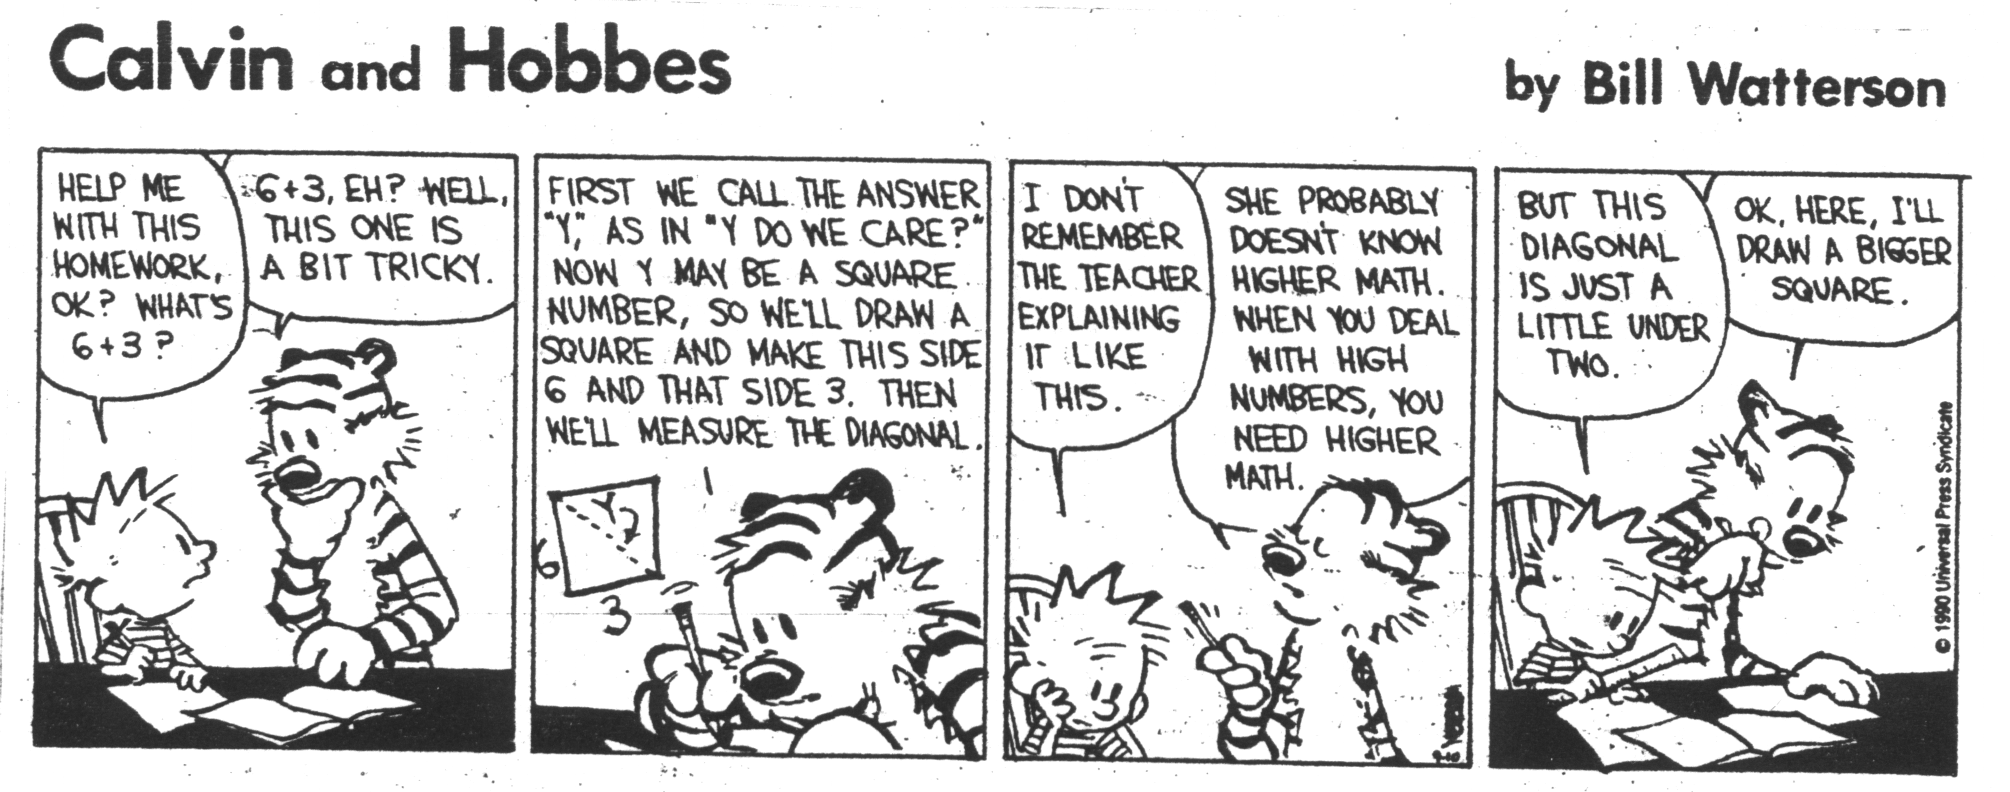
\includegraphics[width=0.8\textwidth]{hobbes}
\end{center}

\subsection*{What is mathematical proof?}
A proof, that is, a mathematical argument, is a work of fiction, a poem. Its goal is to satisfy. A beautiful proof should explain, and it should explain clearly, deeply, and elegantly. A well-written, well-crafted argument should feel like a splash of cool water, and be a beacon of light --- it should refresh the spirit and illuminate the mind. And it should be charming.
\begin{flushright}--- From \emph{A Mathematician's Lament}, by Paul Lockhart.\end{flushright}

Mathematics is fantastic. It is a subject where we do not have to take anyone’s word or
opinion. The truth is not determined by a higher authority who says ‘because I say so’,
or because they saw it in a dream, the pixies at the bottom of their garden told them, or
it came from some ancient mystical tradition. The truth is determined and justified with a
mathematical proof.

A proof is an explanation of why a statement is true. More properly it is a convincing
explanation of why the statement is true. By convincing I mean that it is convincing to
a mathematician. (What that means is an important philosophical point which I am not
going to get into; my interest is more in practical matters.)

Statements are usually proved by starting with some obvious statements, and proceeding
by using small logical steps and applying definitions, axioms and previously established
statements until the required statement results.

The mathematician’s concept of proof is different to everyday usage. In everyday usage
or in court for instance, proof is evidence that something is likely to be true. Mathematicians
require more than this. We like to be 100\% confident that a statement has been proved.
We do not like to be ‘almost certain’.

Having said that, how confident can we be that a theorem has been proved? Millions
have seen a proof of Pythagoras’ Theorem; we can be certain it is true. Proofs of newer
results, however, may contain mistakes. I know from my own experience that some proofs
given in books and research journals are in fact wrong.

\begin{flushright}
  --- From \textit{How to Think Like a Mathematician}, by Kevin Houston.
\end{flushright}

\subsection*{Why am I expected to prove things?}
As a student, you are expected to (try to) learn to think like a mathematician --- and that means to
justify and prove things. Some students (hopefully not you) think that this is somehow too
hard: that being expected to think creatively is something that is best left out of the mathematics
classroom. For that student, I give a number of reasons for the fact (and it is a fact) that
creative mathematical thinking is both possible and necessary for the secondary school student.
\begin{enumerate}
  \item If we don't justify our statements, or understand what we are doing, and simply plug numbers
        into a formula we are doing then we are not only not doing mathematics, but we are wasting
        our time! If mathematics was just about plugging numbers into formulae, we wouldn't bother
        teaching it to students --- because computers are far more reliable, and complain far less. You
        should be aiming to understand \emph{why}, not simply to memorise \emph{how}: and the idea
        of a proof is to \emph{explain the why}.
  \item As Paul Lockhart puts it in his classic book \textit{A Mathematician's Lament}, we believe that
        secondary students are mature enough to have sophisticated opinions on literature and creative
        enough to be allowed to paint, write, and create music; so it isn't really a stretch to believe
        that secondary students are capable of doing their own mathematics.
  \item A good argument is aesthetic (as some of you, who may be considering going to university to study law,
        literature, or another art, will well be aware); mathematicians have a reasonably well-developed idea
        of an aesthetic mathematical argument or mathematical theory, and it is accessible to you. Mathematics
        is one of the oldest forms of human expression, and some of the most elegant proofs that you will
        meet this year date back at least as far as the Greeks --- and over the coming years, you will meet
        modern proofs in subjects that have a different aesthetic nature to (say) geometry.
  \item A (correct) mathematical proof is absolute and forever, in that if a mathematical statement is proved
        then it cannot be overturned in thirty years like a theory of chemistry or biology might be upon the
        discovery of hitherto unknown evidence. Mathematical reasoning is not empirical (based simply on observation
        and the collection of evidence), it is based on logical inference and argument.
  \item Mathematical reasoning is important in other artistic disciplines (history, linguistics, philosophy) and
        in the scientific disciplines (physics, chemistry, biology) --- and is particulary intertwined with
        computer science.
\end{enumerate}

\subsection*{Homework expectations}
For each topic there is a page of homework, usually a piece of reading or a video with a few questions. In addition,
it will be highly adventageous for you to keep up with reading the notes as we go along. \emph{It is your responsibility
to do the homework and to keep up with the notes.} By this last statement I mean, if you have questions, or trouble,
or you're getting things confused, or you forget things, \emph{let me know and we will work through them}.

I am hesitant to recommend a specific length of time that you should be spending on the homework problems because this varies from
person to person. You should be spending enough time that you have a good attempt at each problem --- by which I mean, you have at
least identified what kind of techniques might be applicable, and you have tried to apply them.

\paragraph{What you get out of the homework}
\begin{itemize}
  \item An opportunity to practice the material we cover.
  \item A different perspective on the subject (from the readings).
  \item A chance for you to think things through on your own.
  \item A way to test your own knowledge.
  \item And a baseline for the kinds of things you are expected to be able to do by the end of each topic.
\end{itemize}

\subsection*{Some advice}
\begin{itemize}
  \item Draw pictures, even if you are not strictly doing ``geometry''.
  \item Take the time to write clearly and slowly, because a piece of mathematics that is not clear and transparent to the
        reader is not mathematics at all.
  \item Always ask `why', because nothing is every arbitrary: there will be a reason for everything, even if it is not
        explicitly spelled out in the notes. Ask why things are true, ask why particular problems are in the notes (because
        most of them have a particular goal, or a particular idea to illustrate that may not be immediately obvious).
  \item If you don't understand something (and by `understand' I mean \emph{really understand}, in that you can `see' it
        in your mind and it has become almost obvious), ask questions and try to see things from another perspective.
  \item If you try a problem and you can't see a way through it immediately, come back later; usually, there is not an `answer'
        that is to be calculated, but a process to be discovered or an argument to be developed --- and it sometimes takes time
        for your mind to think unconsciously.
  \item Spend time on problems you think you can't do, because usually there is only a small flash of inspiration required;
        and anyway, the more difficult problems are far more interesting than the `punch some buttons on the calculator' exercises,
        because they have a deeper meaning and are far more satisfying to complete. You might even surprise yourself.
  \item Always try to generalise: sure, it works for right-angled triangles: but what about \emph{all} triangles?
\end{itemize}

The key is not calculations, it is comprehension. Calculations about triangles are not interesting, but the fact that such calculations
are possible is not only interesting but almost counterintuitive; solving a quadratic equation is not interesting, but the idea of
completing the square is interesting because it almost shouldn't work; and taking derivatives is not interesting, but the notion
of describing geometry in a smooth and continuous way is, because it highlights the completeness of our number system. Look for the
counterintuitive, not the boring routine; and try to see the beauty behind the arguments.

Good luck.

\begin{center}
  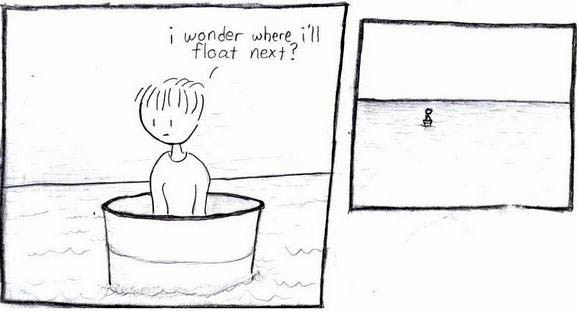
\includegraphics[width=0.8\textwidth]{barrel}
\end{center}
\begin{flushright}--- \url{https://www.xkcd.com/1/}\end{flushright}

\end{document}
